% !TeX spellcheck = en_US
% !TeX encoding = utf8
% !TeX program = xelatex
% !BIB program = bibtex

\documentclass[notes]{beamer}
% \documentclass[draft]{beamer}	
\usetheme{Singapore}
% \usecolortheme{default}
%\usepackage{pgfpages}
%\setbeameroption{show notes on second screen}

\usepackage[british]{babel}
\usepackage{graphicx,hyperref,url}
% \usepackage{ru}
\usepackage{mmstyles}
% \usepackage{hanging}
\usepackage{listings}
\usepackage{fontspec}
\usefonttheme[onlymath]{serif}
\usepackage{xeCJK}
% \usepackage[backend=biber]{biblatex}
% \bibliography{./ref.bib}
%\addbibresource{ref.bib}
\usepackage{indentfirst}
\usepackage{longtable}
\usepackage{float}
%\usepackage{picins}
\usepackage{rotating}
\usepackage{subfigure}
\usepackage{tabu}
\usepackage{amsmath}
\usepackage{amssymb}
\usepackage{setspace}
\usepackage{amsfonts}
\usepackage{appendix}
\usepackage{listings}
\usepackage{xcolor}
\usepackage{geometry}
% \setCJKfamilyfont{cjkhwxk}{SimSun}
% \newcommand*{\cjkhwxk}{\CJKfamily{cjkhwxk}}
%\newfontfamily{\consolas}{Consolas}
%\newfontfamily{\monaco}{Monaco}
%\setmonofont[Mapping={}]{Consolas}	%英文引号之类的正常显示,相当于设置英文字体
%\setsansfont{Consolas} %设置英文字体 Monaco, Consolas,  Fantasque Sans Mono
% \setmainfont{Times New Roman}
% \newfontfamily{\consolas}{Times New Roman}
% \newfontfamily{\monaco}{Arial}
% \setCJKmainfont{Times New Roman}
%\setmainfont{MONACO.TTF}
%\setsansfont{MONACO.TTF}
\newcommand{\verylarge}{\fontsize{60pt}{\baselineskip}\selectfont}  
\newcommand{\chuhao}{\fontsize{44.9pt}{\baselineskip}\selectfont}  
\newcommand{\xiaochu}{\fontsize{38.5pt}{\baselineskip}\selectfont}  
\newcommand{\yihao}{\fontsize{27.8pt}{\baselineskip}\selectfont}  
\newcommand{\xiaoyi}{\fontsize{25.7pt}{\baselineskip}\selectfont}  
\newcommand{\erhao}{\fontsize{23.5pt}{\baselineskip}\selectfont}  
\newcommand{\xiaoerhao}{\fontsize{19.3pt}{\baselineskip}\selectfont} 
\newcommand{\sihao}{\fontsize{14pt}{\baselineskip}\selectfont}      % 字号设置  
\newcommand{\xiaosihao}{\fontsize{12pt}{\baselineskip}\selectfont}  % 字号设置  
\newcommand{\wuhao}{\fontsize{10.5pt}{\baselineskip}\selectfont}    % 字号设置  
\newcommand{\xiaowuhao}{\fontsize{9pt}{\baselineskip}\selectfont}   % 字号设置  
\newcommand{\liuhao}{\fontsize{7.875pt}{\baselineskip}\selectfont}  % 字号设置  
\newcommand{\qihao}{\fontsize{5.25pt}{\baselineskip}\selectfont}    % 字号设置 

\graphicspath{{./fig/}}

% \setbeamertemplate{footnote}{%
%   \hangpara{2em}{1}%
%   \makebox[2em][l]{\insertfootnotemark}\footnotesize\insertfootnotetext\par%
% }

\definecolor{cred}{rgb}{0.6,0,0}
\definecolor{cgreen}{rgb}{0.25,0.5,0.35}
\definecolor{cpurple}{rgb}{0.5,0,0.35}
\definecolor{cdocblue}{rgb}{0.25,0.35,0.75}
\definecolor{cdark}{rgb}{0.95,1.0,1.0}
\lstset{
	language=R,
	numbers=left,
	numberstyle=\tiny\color{black},
	keywordstyle=\color{cpurple}\consolas,
	commentstyle=\color{cgreen}\consolas,
	stringstyle=\color{cred}\consolas,
	frame=single,
	escapeinside=``,
	xleftmargin=1em,
	xrightmargin=1em, 
	backgroundcolor=\color{cdark},
	aboveskip=1em,
	breaklines=true,
	tabsize=3
} 
% The title of the presentation:
%  - first a short version which is visible at the bottom of each slide;
%  - second the full title shown on the title slide;
\title[adalimumab]{Adaptive Multi-Column Deep Neural Networks with Application to Robust Image Denoising}

% % Optional: a subtitle to be dispalyed on the title slide
% \subtitle{Optimization for Biosensor}

% % The author(s) of the presentation:
% %  - again first a short version to be displayed at the bottom;
% %  - next the full list of authors, which may include contact information;
\author[Zejia LV]{Zejia LV \\ zejialv@zju.edu.cn}
% % The institute:
% %  - to start the name of the university as displayed on the top of each slide
% %    this can be adjusted such that you can also create a Dutch version
% %  - next the institute information as displayed on the title slide

%\institute[, ZJU]{, ZJU}

% Add a date and possibly the name of the event to the slides
%  - again first a short version to be shown at the bottom of each slide
%  - second the full date and event name for the title slide
\date[\today]{\today}

\begin{document}

\AtBeginSection[]
{
	\begin{frame}
		\frametitle{Outline}
		\tableofcontents[currentsection]
	\end{frame}
}
\begin{frame}
	\titlepage
\end{frame}


\begin{frame}{Introduction}
	\begin{block}{Background}
		Digital images are often corrupted with noise during the acquisition and transmission, disgrading performance in the later tasks such as: image recognition and medical diagnosis. But traditional denoising algorithms are carefully designed for certain type of noise or require assumptions about the statistical properties of corrupting noise.	
	\end{block}	
	\begin{block}{What we do}
		We demonstrate the Adaptive Multi-Column sparse stacked denoising autoencoder(AMC-SSDA), a method to improve the SSDA's robustness to various noise types and provides better denoising results for both noise types presents in the training set and for noise types not seen by denoiser during training(which means we eliminate the need to determine the types of noise and let alone its statistics at test time). Additionally, strong classification performance has been achieved on corrupted MNIST digits.
	\end{block}
\end{frame}

\begin{frame}{Algorithms}
	\begin{block}{Stacked sparse denoising autoencoders}
	 We can define the Feedforward functions as follows:
		\begin{equation}
			\begin{split}
				\mathbf { h } ( \mathbf { x } ) = f ( \mathbf { W } \mathbf { x } + \mathbf { b } )
			\end{split}
		\end{equation}
		\begin{equation}
			\begin{split}
				\hat { \mathbf { y } } ( \mathbf { x } ) = g \left( \mathbf { W } ^ { \prime } \mathbf { h } + \mathbf { b } ^ { \prime } \right)
			\end{split}
		\end{equation}
		for encoding and decoding functions:
		\begin{equation}
			\begin{split}
				\sigma ( s ) = \frac { 1 } { 1 + \exp ( - s ) }
			\end{split}
		\end{equation}
		
	\end{block}
\end{frame}


\begin{frame}{Algorithms}
	\begin{block}{Stacked sparse denoising autoencoders}
		\begin{figure}
			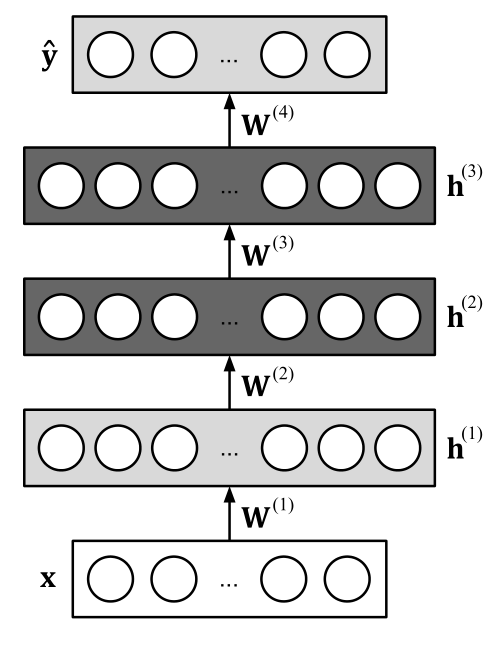
\includegraphics[width=0.4\textwidth]{1.png}
		\end{figure}
	\end{block}
\end{frame}


\begin{frame}{Algorithms}
	\begin{block}{Stacked sparse denoising autoencoders}
		The DA is trained by backpropagation to minimize the sparsity reqularized reconstruction loss gived by:
		\begin{small}
			\begin{equation}
			\begin{split}
				\mathcal { L } _ { \mathrm { DA } } ( \mathcal { D } ;  \Theta  ) &= \frac { 1 } { N } \sum _ { i = 1 } ^ { N } \left\| \mathbf { y } _ { i } - \hat { \mathbf { y } } \left( \mathbf { x } _ { i } \right) \right\| _ { 2 } ^ { 2 } + \beta \sum _ { j = 1 } ^ { K } \mathrm { KL } ( \rho \| \hat { \rho } _ { j } ) + \frac { \lambda } { 2 } \left( \| \mathbf { W } \| _ { \mathrm { F } } ^ { 2 } + \left\| \mathbf { W } ^ { \prime } \right\| _ { \mathrm { F } } ^ { 2 } \right) \\
				 \Theta& = \left\{ \mathbf { W } , \mathbf { b } , \mathbf { W } ^ { \prime } , \mathbf { b } ^ { \prime } \right\}
			\end{split}
		\end{equation}
		\end{small}
		 Kullback-Leibler divergence:
		 \begin{small}
		 	 \begin{equation}
		 	\begin{split}
		 		\mathrm { KL } \left( \hat { \rho } _ { j } \| \rho \right) = \rho \log \frac { \rho } { \hat { \rho } _ { j } } + ( 1 - \rho ) \log \frac { ( 1 - \rho ) } { 1 - \hat { \rho } _ { j } } \quad \text { where } \quad \hat { \rho } _ { j } = \frac { 1 } { N } \sum _ { i = 1 } ^ { N } h _ { j } \left( \mathbf { x } _ { i } \right)
		 	\end{split}
		 \end{equation}
		 \end{small}
	\end{block}
\end{frame}


\begin{frame}{Algorithms}
	\begin{block}{Stacked sparse denoising autoencoders}
		For SSDA
		 \begin{small}
		 	 \begin{equation}
		 	\begin{split}
		 		L _ { \mathrm { SSDA } } ( \mathcal { D } ;\Theta \mathbf { \Theta } ) = \frac { 1 } { N } \sum _ { i = 1 } ^ { N } \left\| \mathbf { y } _ { i } - \hat { \mathbf { y } } \left( \mathbf { x } _ { i } \right) \right\| _ { 2 } ^ { 2 } + \frac { \lambda } { 2 } \sum _ { l = 1 } ^ { 2 L } \left\| \mathbf { W } ^ { ( l ) } \right\| _ { \mathrm { F } } ^ { 2 }
		 	\end{split}
		 \end{equation}
		 \end{small}
	\end{block}
\end{frame}

\begin{frame}{Algorithms}
	\begin{block}{Adaptive Multi-Column SSDA}
	AMC-SSDA is the linear combination of serveral SSDAs, or \textbf{columns}, each trained on a single type of noise using optimized weights determined by the features of each given input image.
		\begin{figure}
		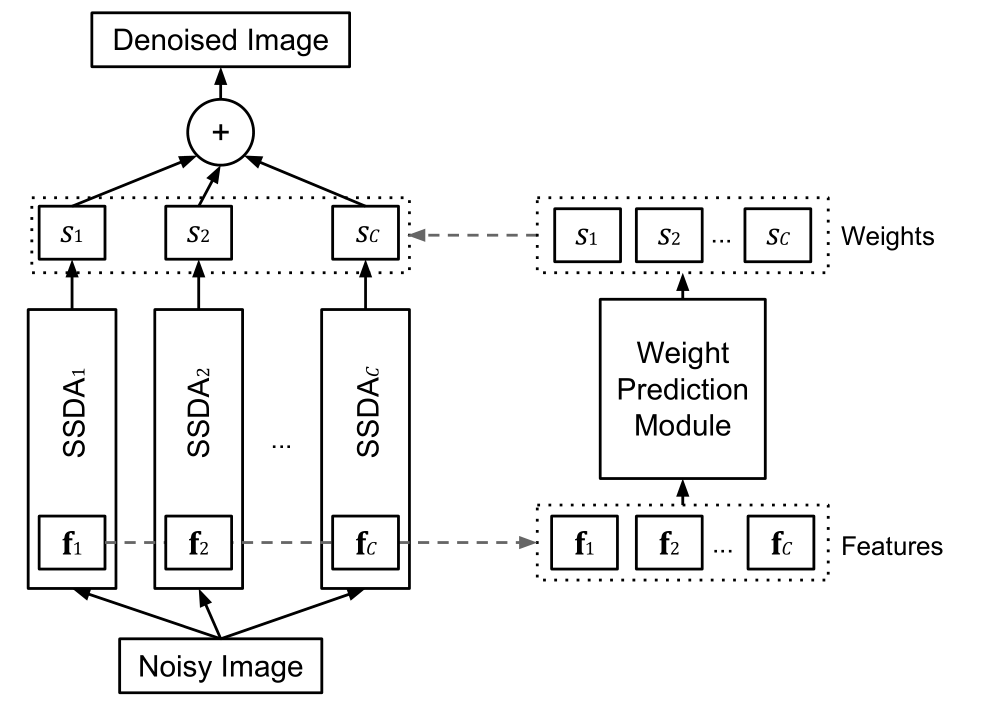
\includegraphics[width=0.6\textwidth]{2.png}
	\end{figure}
	\end{block}
\end{frame}


\begin{frame}{Algorithms}
	\begin{block}{Adaptive Multi-Column SSDA}
		 \begin{small}
		 	 \begin{equation}
		 	\begin{split}
		 	\text { minimize } _ { \left\{ s _ { c } \right\} } \quad &\frac { 1 } { 2 } \left\| \hat { \mathbf { Y } } _ { \mathbf { S } } - \mathbf { y } \right\| ^ { 2 }\\
		 	\text { subject to } \quad &0 \leq s _ { c } \leq 1 , \forall c\\
		 	&1 - \delta \leq \sum _ { c = 1 } ^ { C } s _ { c } \leq 1 + \delta
		 	\end{split}
		 \end{equation}
		 \end{small}
		 Learning to predict optimal column weights via RBF Networks
	\end{block}
\end{frame}

\begin{frame}{Experiments}
	\begin{block}{Visualization of denoising performance}
		\begin{figure}
			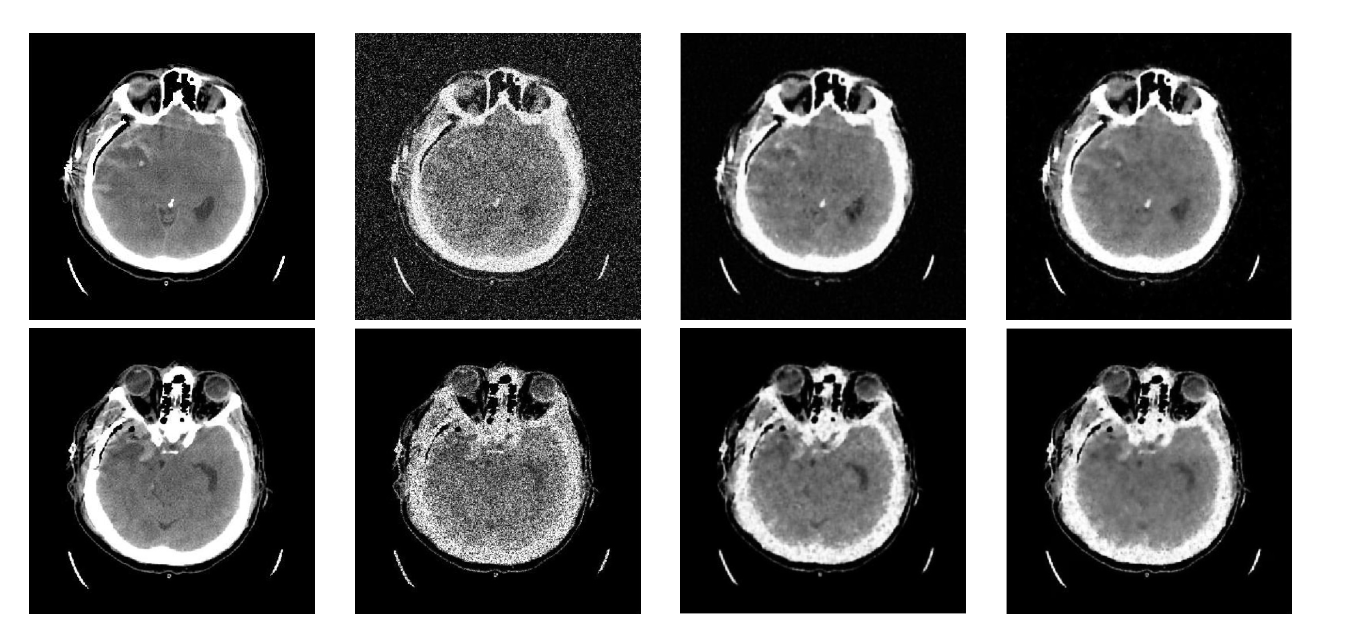
\includegraphics[width=0.6\textwidth]{3.png}
		\end{figure}
	\end{block}
\end{frame}

\begin{frame}{Experiments}
	\begin{block}{MNIST test classification error of denoised images}
		\begin{figure}
			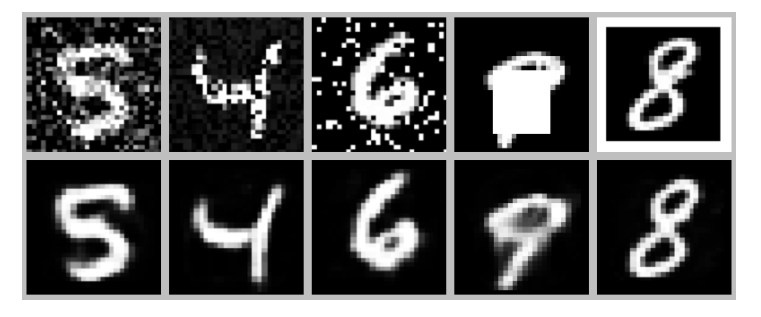
\includegraphics[width=0.4\textwidth]{4.png}
		\end{figure}
		\begin{figure}
			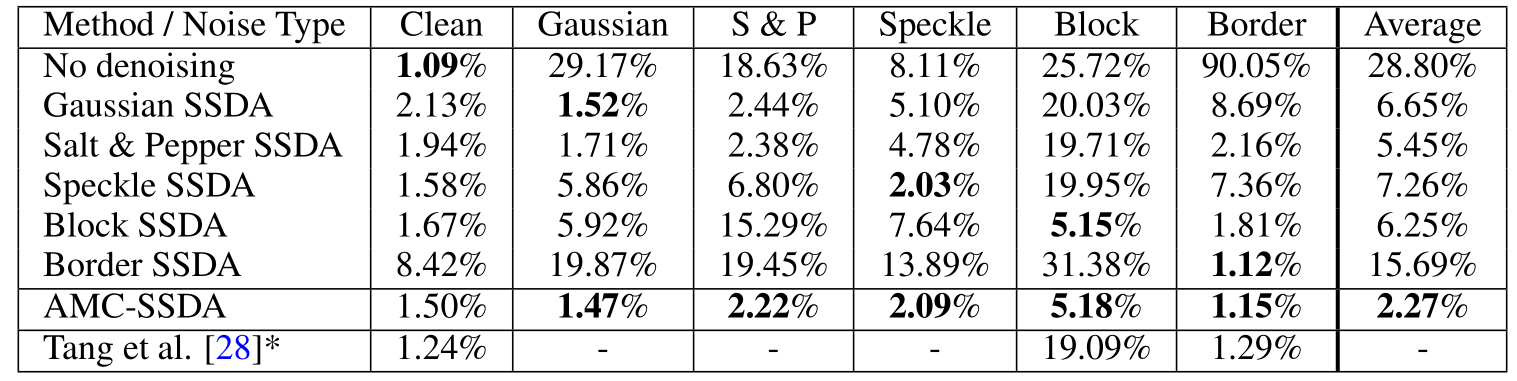
\includegraphics[width=1.0\textwidth]{5.png}
		\end{figure}
	\end{block}
\end{frame}

\begin{frame}{Further}
	\begin{block}{Ongoing Optimization}
		\begin{itemize}
			\item Maybe analysis time limits?
		\end{itemize}
	\end{block}
\end{frame}


\begin{frame}{References}
	\begin{itemize}
		\item Forest Agostinelli Michael R. Anderson Honglak Lee. \textit{Adaptive Multi-Column Deep Neural Networks
with Application to Robust Image Denoising}
	
	\end{itemize}
\end{frame}




\end{document}
